\section{\lr{Page Cache}}
به نظر من بهتر است که در ابتدا خارج از برنامه فایل مذکور را ساخته و سپس بعد برنامه‌ای بنویسیم که فقط خواندن و سپس
فقط نوشتن را انجام دهد. برای بیشتر حس شدن تاثیر
\lr{read} و \lr{write}
من با اینکه سیستم خودم بر روی
\lr{nVME}
نصب است ولی بر روی یک هارد دیسک دیتا را ذخیره می‌کنم که کند باشد. این پارتیشن با فایل سیستم
\lr{ext4}
فرمت شده است.

برای ساختن فایل از دستور زیر استفاده می‌کنیم:
\samplebox{dd if=/dev/urandom of=/media/hirbod/LinuxHDD/sample.dat count=10240 bs=1M}
سرعت نوشتن این فایل با توجه به
\codeword{dd}
برابر 92 مگابایت است.
\begin{figure}[H]
    \centering
    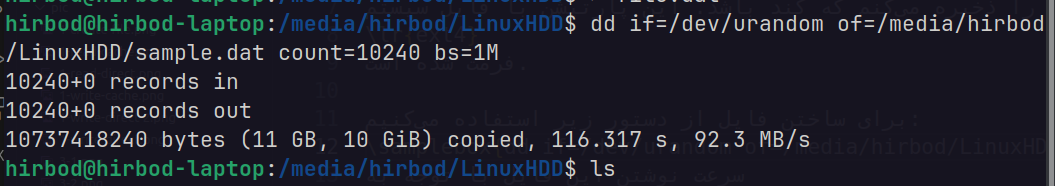
\includegraphics[scale=0.4]{pic/1-dd.png}
    \caption{نوشتن در دیسک به کمک \lr{dd}}
\end{figure}


سپس به کمک برنامه فایل را با
\lr{cache}
10 بار می‌خوانیم.
زمان اجرای برنامه به صورت زیر است:
\samplebox{real    2m48.880s\\
user    0m1.650s\\
sys     0m28.315s} % Read Cache

حال
\lr{cache}
را غیر فعال می‌کنیم. سرعت خواندن به صورت زیر می‌شود. این عدد نشان می‌دهد که سرعت خواندن حدودا برابر
$\frac{1024 \times 1024 \times 1024 \times 10 \times 10}{26 \times 60 + 16} \approx 65 MB/s$
است.
\samplebox{real    26m16.402s\\
user    0m10.612s\\
sys     2m41.620s} % Read Direct
اما خواندن فایل به این سادگی‌ها نبود! یک مشکلی که من داشتم این بود که زمانی که
\codeword{read}
را صدا می‌زدم به ارور
\codeword{EINVAL}
می‌خوردم. با خواندن
\lr{man page}
\codeword{read}
به خط زیر بر می‌خوریم:
\begin{latin}
\begin{quote}
    \textbf{EINVAL}: fd is attached to an object which is unsuitable for reading; or the file was opened with the O\_DIRECT flag, and either the address specified in buf,
    the value specified in count, or the file offset is not suitably aligned.
\end{quote}
\end{latin}
همان طور که مشخص است باید زمانی که از
\lr{direct io}
استفاده می‌کنیم مموری که می‌خواهیم در آن بخوانیم
\lr{page aligned}
باشد و حتی سایز آن نیز باید مضرب \lr{page size} باشد. پس به کمک دستور
\codeword{posix\_memalign}
مموری بافر را می‌گیریم.

همچنین برای نمونه من بعد از زدن تست
\lr{cached read}
باری دیگر بدون پاک کردن کش همان برنامه را اجرا کردم. زمان اجرای برنامه به صورت زیر است که نشان می‌دهد که
کلا سیستم عامل با دیسک دیگر کاری ندارد.
\samplebox{real    0m9.235s\\
user    0m0.917s\\
sys     0m8.317s}

حال طیق خواسته‌ی قسمت دوم سوال برنامه را بدون زدن دستورات پاک کردن کش با
\lr{direct IO}
اجرا می‌کنیم. زمان اجرا به صورت زیر است:
\samplebox{real    25m22.122s\\
user    0m11.894s\\
sys     3m2.843s}
همان طور که مشاهده می‌شود تفاوت آنچنانی بین زمانی که کش را پاک کردیم و نکردیم وجود ندارد.

حال سرعت نوشتن با کش را تست می‌کنیم. با توجه به نتیجه‌ی زیر سرعت آن حدود
$59.5 MB/s$
است.
\samplebox{real    30m6.216s\\
user    0m3.986s\\
sys     4m11.283s} % Write Cache

در ادامه سعی کردم که دقیقا همین تست را با
\lr{direct IO}
تست کنم. اما یک مشکلی وجود داشت\dots
برنامه خیلی خیلی در حال طول کشیدن بودن. من یک ساعت و نیم صبر کردم ولی دیدم که برنامه تمام نمی‌شود. پس یک سری
پیام دیباگ اضافه کردم که بگوید که در
\lr{iteration}
چندم است. با این حال نیز دیدم برنامه خیلی در حال طول کشیدن است. پس از
\lr{htop}
استفاده کردم که چک کنیم که سرعت نوشتن چه قدر است و نتیجه شکل
\ref{fig:direct_io_write_speed}
شد.
\begin{figure}[H]
    \centering
    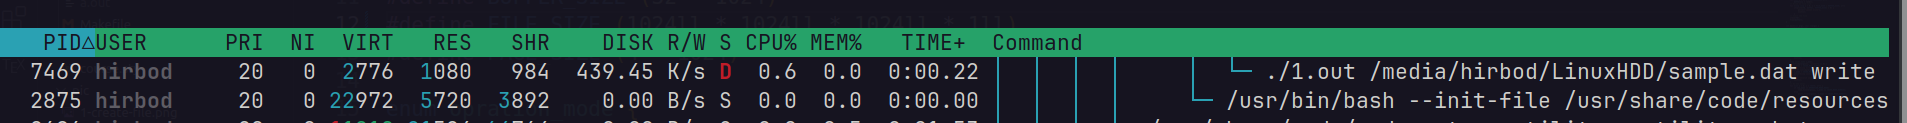
\includegraphics[scale=0.3]{pic/1-write-direct.png}
    \caption{سرعت نوشتن در حالت \lr{direct IO}}
    \label{fig:direct_io_write_speed}
\end{figure}

به خاطر سرعت پایین آن من کمی صورت آزمایش را عوض کردم و حجم فایل را به 8 مگابایت کاهش دادم. سرعت اجرای برنامه به صورت
زیر شد:


\smalltitle{\lr{Cached Write}:}
\samplebox{real    0m0.710s\\
user    0m0.025s\\
sys     0m0.252s}

\smalltitle{\lr{Direct Write}:}
\samplebox{real    1m2.256s\\
user    0m0.044s\\
sys     0m0.443s}

حال بررسی می‌کنیم که سرعت در نوشتن بیشتر بیشتر می‌شود یا خواندن. متوجه می‌شویم که در خواندن حالت
\lr{cache}
سرعت خواندن را حدودا 13 برابر بیشتر می‌کند. ولی در نوشتن سرعت خواندن حدود 88 برابر می‌شود!
پس تاثیر آن بر روی نوشتن بیشتر است. یکی از دلیل‌های آن می‌تواند این باشد که در نوشتن سیستم‌عامل حتی مطمئن می‌شود که
از کش خود هارد نیز استفاده نشود. چرا که سرعت 500 کیلوبایت بر ثانیه حدودا برابر سرعت
\lr{random read/write}
در
\lr{HDD}
است.